\documentclass[tikz,border=8pt]{standalone}
\usepackage{amsmath}
\usetikzlibrary{arrows.meta}

\begin{document}
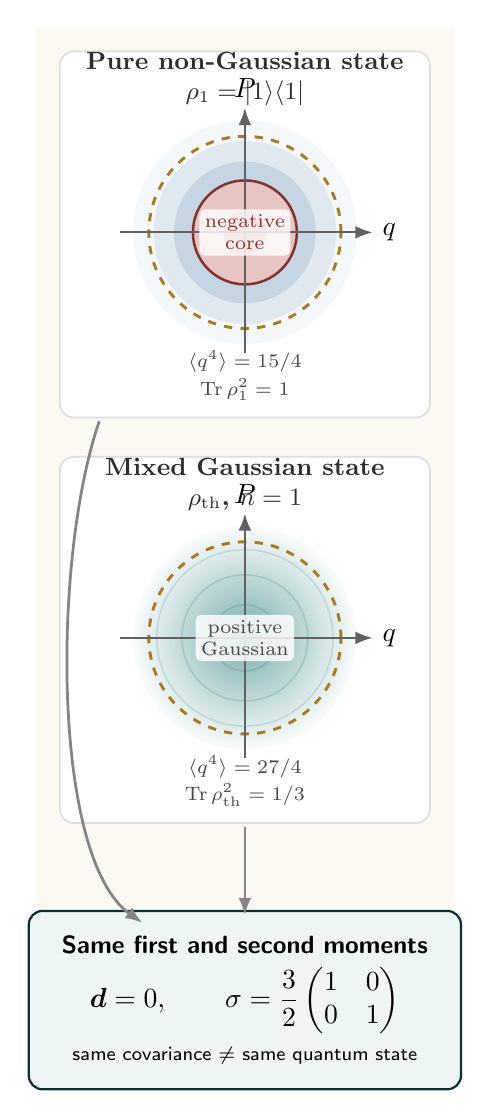
\begin{tikzpicture}[
  >=Latex,
  font=\sffamily,
  axis/.style={->,line width=.7pt,draw=black!62},
  flow/.style={-{Latex[length=2.2mm]},line width=1pt,draw=black!48},
  heading/.style={font=\small\bfseries,text=black!82,align=center},
  note/.style={font=\scriptsize,text=black!72,align=center},
  result/.style={rounded corners=5pt,draw=teal!45!black,fill=teal!7,
    line width=.8pt,inner xsep=12pt,inner ysep=9pt,align=center}
]

\definecolor{paper}{RGB}{252,249,243}
\definecolor{teal}{RGB}{16,111,108}
\definecolor{blue}{RGB}{54,111,153}
\definecolor{red}{RGB}{176,67,62}
\definecolor{gold}{RGB}{202,145,37}

\fill[paper] (-2.65,-5.85) rectangle (2.65,7.55);

\fill[white,rounded corners=5pt] (-2.35,2.60) rectangle (2.35,7.25);
\draw[black!13,rounded corners=5pt,line width=.6pt]
  (-2.35,2.60) rectangle (2.35,7.25);

\fill[white,rounded corners=5pt] (-2.35,-2.55) rectangle (2.35,2.10);
\draw[black!13,rounded corners=5pt,line width=.6pt]
  (-2.35,-2.55) rectangle (2.35,2.10);

% Non-Gaussian first excited state
\begin{scope}[shift={(0,4.95)}]
  \node[heading] at (0,1.95)
    {Pure non-Gaussian state\\$\rho_1=\lvert1\rangle\langle1\rvert$};

  \fill[blue!5] (0,0) circle (1.42);
  \fill[blue!15] (0,0) circle (1.16);
  \fill[blue!29] (0,0) circle (.90);
  \fill[red!31] (0,0) circle (.66);
  \fill[red!58] (0,0) circle (.27);
  \draw[red!75!black,line width=.9pt] (0,0) circle (.66);
  \draw[gold!84!black,dashed,line width=1.05pt] (0,0) circle (1.22);

  \draw[axis] (-1.58,0) -- (1.62,0) node[right] {$q$};
  \draw[axis] (0,-1.53) -- (0,1.58) node[above] {$P$};

  \node[note,text=red!78!black,fill=white,fill opacity=.82,text opacity=1,
    rounded corners=2pt,inner sep=2pt] at (0,0)
    {negative\\core};
  \node[note] at (0,-1.82)
    {$\langle q^4\rangle=15/4$\\[2pt]
     $\operatorname{Tr}\rho_1^2=1$};
\end{scope}

% Gaussian thermal state
\begin{scope}[shift={(0,-.20)}]
  \node[heading] at (0,1.95)
    {Mixed Gaussian state\\$\rho_{\mathrm{th}}$, \(\bar n=1\)};

  \shade[inner color=teal!57,outer color=teal!2]
    (0,0) circle (1.42);
  \draw[teal!52,line width=.55pt] (0,0) circle (.42);
  \draw[teal!40,line width=.55pt] (0,0) circle (.80);
  \draw[teal!27,line width=.55pt] (0,0) circle (1.12);
  \draw[gold!84!black,dashed,line width=1.05pt] (0,0) circle (1.22);

  \draw[axis] (-1.58,0) -- (1.62,0) node[right] {$q$};
  \draw[axis] (0,-1.53) -- (0,1.58) node[above] {$P$};

  \node[note,fill=white,fill opacity=.82,text opacity=1,
    rounded corners=2pt,inner sep=2pt] at (0,0)
    {positive\\Gaussian};
  \node[note] at (0,-1.82)
    {$\langle q^4\rangle=27/4$\\[2pt]
     $\operatorname{Tr}\rho_{\mathrm{th}}^2=1/3$};
\end{scope}

\node[result] (same) at (0,-4.80)
  {{\small\bfseries Same first and second moments}\\[4pt]
   $\boldsymbol d=0,\qquad
    \sigma=\dfrac32
    \begin{pmatrix}1&0\\0&1\end{pmatrix}$\\[4pt]
   {\scriptsize same covariance \(\neq\) same quantum state}};

\draw[flow] (-1.85,2.55) .. controls (-2.45,.80) and (-2.45,-3.00) ..
  (-1.30,-3.82);
\draw[flow] (0,-2.60) -- (0,-3.72);

\end{tikzpicture}
\end{document}
